\section{Adjugate Matrices}

\subsection{Column and row expansions}
Let $A \in M_n(F)$ with column vectors $A^{(i)}$.
We know that
\begin{align*}
	\det(A^{(1)}, \dots, A^{(j)}, \dots, A^{(k)}, \dots, A^{(n)}) = -\det(A^{(1)}, \dots, A^{(k)}, \dots, A^{(j)}, \dots, A^{(n)})
\end{align*}
Using the fact that $\det A = \det A^\transpose$ we can similarly see that swapping two rows will invert the sign of the determinant.
\begin{remark}
	We could have proven all of the properties of the determinant above by using the decomposition of $A$ into elementary matrices.
\end{remark}
\begin{definition}[Minor]
	Let $A \in M_n(F)$.
	Let $i, j \in \qty{1, \dots, n}$.
	We define the \vocab{minor} $A_{\widehat{ij}} \in M_{n-1}(F)$ to be the matrix obtained by removing the $i$th row and the $j$th column from $A$.
\end{definition}

\begin{example} ~\vspace*{-1.5\baselineskip}
	\begin{align*}
		A &= \begin{pmatrix}1 & 2 & -7 \\2 & 1 & 0 \\-3 & 6 & 1\end{pmatrix} \\
		A_{\widehat{32}} &= \begin{pmatrix}1 & -7 \\2 & 0\end{pmatrix}
	\end{align*} 
\end{example} 

\begin{lemma}[Expansion of the determinant]
	Let $A \in M_n(F)$.
	\begin{enumerate}
		\item Let $j \in \qty{1, \dots, n}$.
		      The determinant of $A$ is given by the \textit{column expansion with respect to the $j$th column}:
		      \begin{align*}
			      \det A = \sum_{i=1}^n (-1)^{i+j} a_{ij} \det A_{\widehat{ij}}
		      \end{align*}
		\item Let $i \in \qty{1, \dots, n}$.
		      The same determinant is also given by the \textit{row expansion with respect to the $i$th row}:
		      \begin{align*}
			      \det A = \sum_{j=1}^n (-1)^{i+j} a_{ij} \det A_{\widehat{ij}}
		      \end{align*}
	\end{enumerate}
\end{lemma}

This is a process of reducing the computation of $n \times n$ determinants to $(n-1) \times (n-1)$ determinants.
A powerful tool to compute determinants.

\begin{example}
	{\centering 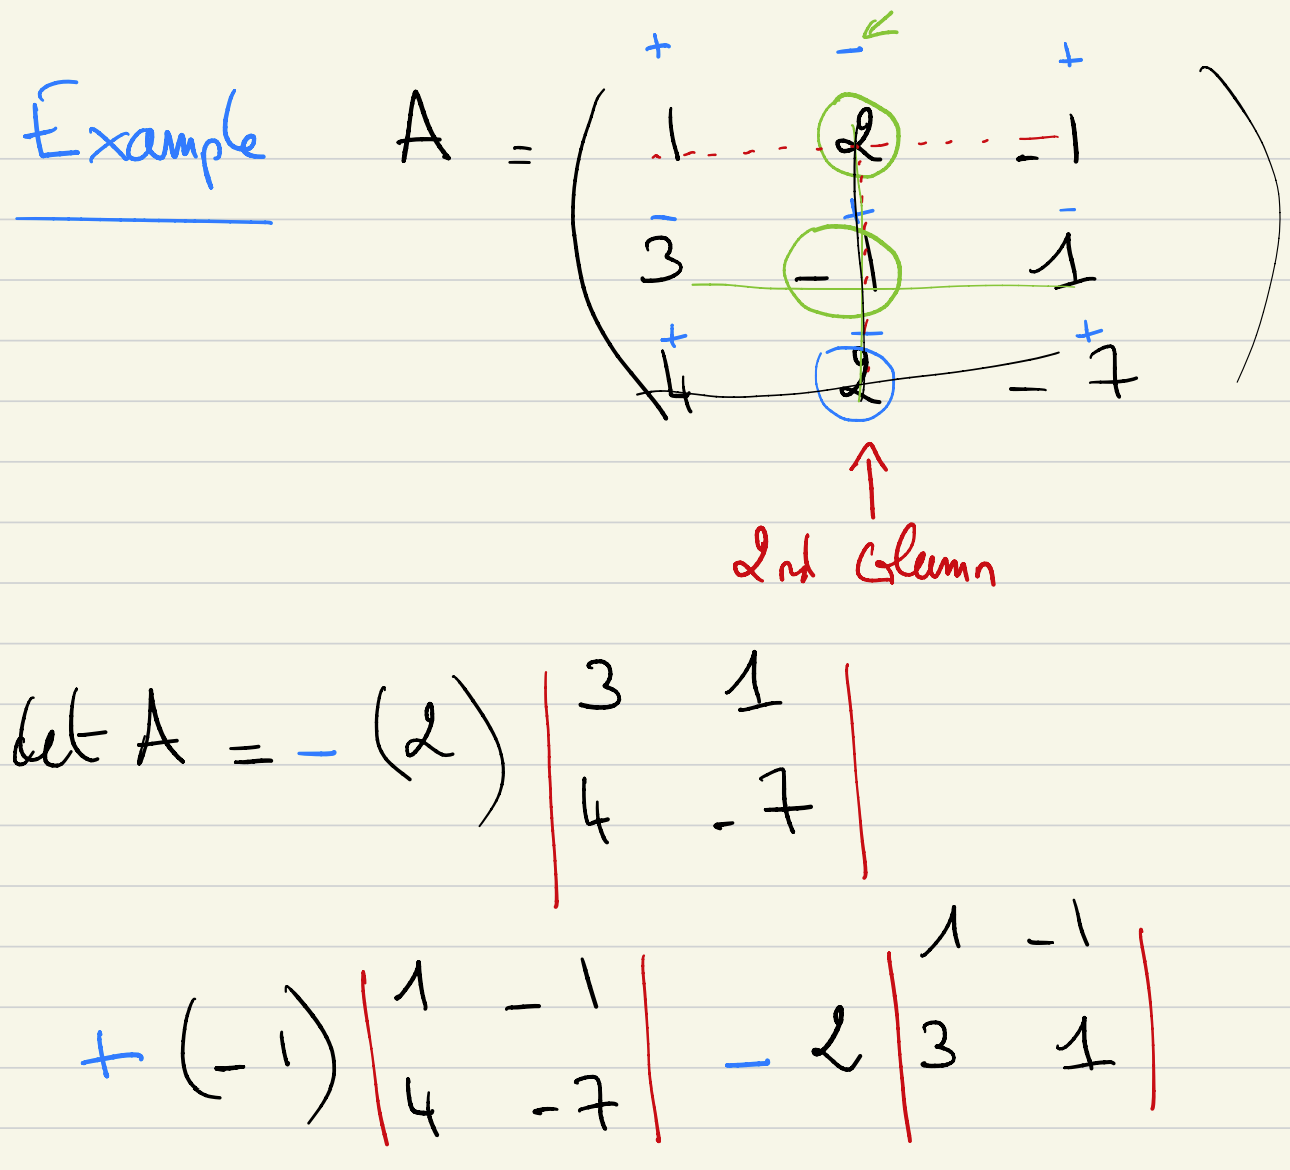
\includegraphics{06-ScreenshotExample.png}}
\end{example} 

\begin{proof}
	We will prove case (i), the column expansion with respect to the $j$th column.
	Then (ii) will follow from the transpose of the matrix.

	Let $j \in \qty{1, \dots, n}$.
	We can write $A^{(j)} = \sum_{i=1}^n a_{ij} e_i$ where the $e_i$ are the canonical basis and $A = (a_{ij})_{1 \leq i, j \leq n}$.
	\begin{align*}
		\det A & = \det\qty(A^{(1)}, \dots, A_{j-1}, \sum_{i=1}^n a_{ij} e_i, A_{j+1}, \dots, A^{(n)}) \\
		& = \sum_{i=1}^n a_{ij} \det\qty(A^{(1)}, \dots, e_i, \dots, A^{(n)})
		\intertext{Then, by swapping rows and columns,}
		& = \sum_{i=1}^n a_{ij} (-1)^{j-1} \det\qty(e_i, A^{(1)}, \dots, A^{(n)}) \\
		\intertext{Swapping the $i$th row with the first:}
		&= \sum_{i=1}^n a_{ij} (-1)^{j-1} (-1)^{i-1} \det \begin{pNiceMatrix}
            1   	& a_{i 1} & \dots & a_{i, j-1}  & a_{i, j+1} & \dots & a_{i n} \\
            0    	&         &\Block{3-4}{A_{\widehat{ij}}}&	&       	 &		 & \\
            \vdots  &         &       &				&       	 &		 & \\
            0	    &         &       &      		&      		 &		 & \\
          \end{pNiceMatrix}\\
	\end{align*}
	This has brought the matrix into block form, where there is an element of value 1 in the top left, and the matrix $A_{\widehat{ij}}$ in the bottom right.
	The bottom left block is entirely zeroes.
	Hence,
	\begin{align*}
		\det A = \sum_{i=1}^n (-1)^{i+j} a_{ij} \det A_{\widehat{ij}}
	\end{align*}
	as required.
\end{proof}
\begin{remark}
	We have proven that
	\begin{align*}
		\det (A^{(1)}, \dots, A_{j-1}, e_i, A_{j+1}, \dots, A^{(n)}) = (-1)^{i+j} \det A_{\widehat{ij}}
	\end{align*}
\end{remark}

\subsection{Adjugates}
\begin{definition}[Adjugate matrix]
	Let $A \in M_n(F)$.
	The \vocab{adjugate matrix} of $A$, denoted $\adj A$, is the $n \times n$ matrix given by
	\begin{align*}
		(\adj A)_{ij} = (-1)^{i+j} \det A_{\widehat{ji}}
	\end{align*}
	Hence,
	\begin{align*}
		\det (A^{(1)}, \dots, A^{(j-1)}, e_i, A^{(j+1)}, \dots, A^{(n)}) = (\adj A)_{ji}
	\end{align*}
\end{definition}

\begin{theorem}
	Let $A \in M_n(F)$.
	Then
	\begin{align*}
		(\adj A) A = (\det A) I
	\end{align*}
	In particular, when $A$ is invertible,
	\begin{align*}
		A^{-1} = \frac{\adj A}{\det A}
	\end{align*}
\end{theorem}

\begin{proof}
	We have
	\begin{align*}
		\det A = \sum_{i=1}^n (-1)^{i+j} a_{ij} \det A_{\widehat{ij}}
	\end{align*}
	Hence,
	\begin{align*}
		\det A = \sum_{i=1}^n (\adj A)_{ji} a_{ij} = ((\adj A) A)_{jj}
	\end{align*}
	So the diagonal terms match.
	Off the diagonal,
	\begin{align*}
		0 = \det(A^{(1)}, \dots, \underbrace{A^{(k)}}_{\mathclap{j\text{th position}}}, \dots, A^{(k)}, \dots, A^{(n)})
	\end{align*}
	By linearity,
	\begin{align*}
		0 &= \det\qty(A^{(1)}, \dots, \underbrace{\sum_{i=1}^n a_{ik} e_i}_{\mathclap{j\text{th position}}}, \dots, A^{(k)}, \dots, A^{(n)}) \\
		&= \sum_{i=1}^n a_{ik} \det\qty(A^{(1)}, \dots, \underbrace{e_i}_{\mathclap{j\text{th position}}}, \dots, A^{(k)}, \dots, A^{(n)}) \\
		&= \sum_{i=1}^n a_{ik} (\adj A)_{ji} \\
		&= ((\adj A) A)_{jk}
	\end{align*}
\end{proof}

\subsection{Cramer's rule}
\begin{proposition}
	Let $A \in M_n(F)$ be invertible.
	Let $b \in F^n$.
	Then the unique solution to $Ax = b$ is given by
	\begin{align*}
		x_i = \frac{1}{\det A} \det (A_{\widehat{ib}})
	\end{align*}
	where $A_{\widehat{ib}}$ is obtained by replacing the $i$th column of $A$ by $b$.
\end{proposition}

This is an algorithm to compute $x$, avoiding the computation of $A^{-1}$.

\begin{proof}
	Let $A$ be invertible.
	Then there exists a unique $x \in F^n$ such that $Ax = b$.
	Then, since the determinant is alternating,
	\begin{align*}
		\det (A_{\widehat{ib}}) &= \det(A^{(1)}, \dots, A^{(i-1)}, b, A^{(i+1)}, \dots, A^{(n)}) \\
		&= \det(A^{(1)}, \dots, A^{(i-1)}, Ax, A^{(i+1)}, \dots, A^{(n)}) \\
		&= \det\qty(A^{(1)}, \dots, A^{(i-1)}, \sum_{j=1}^n x_j A^{(j)}, A^{(i+1)}, \dots, A^{(n)})
		\intertext{As $\det$ linear we can bring out the $x_j$s and then as its alternating,}
		&= x_i \det\qty(A^{(1)}, \dots, A^{(i-1)}, A^{(i)}, A^{(i+1)}, \dots, A^{(n)}) \\
		&= x_i \det A
	\end{align*}
	So the formula works.
\end{proof}